%
\section{Well-formedness Rules of \agl} \label{apex:agl-rules}
%
\subsection{\clazz{ActivityGraph}}
%\ruledef{asmruleno}{R}{graph1}
\begin{lstrule}
-- nodes must contain at least two Nodes
context ActivityGraph inv:
  not(nodes.oclIsUndefined()) and nodes->size()>=2
\end{lstrule}

\begin{lstrule}
-- edges must contain at least one Edge
context ActivityGraph inv:
  not(edges.oclIsUndefined()) and edges->size()>=1
\end{lstrule}

\begin{lstrule}
-- n0 must contain at least one Node and is a subset of nodes
context ActivityGraph inv:
  not(n0.oclIsUndefined()) and nodes->size()>=1 and nodes->includesAll(n0)
\end{lstrule}

\begin{lstrule}
-- (Connectedness) graph is connected (i.e. at least one path connects any two nodes)
context ActivityGraph inv:
  nodes->forAll(n, n' | hasPath(n, n'))
\end{lstrule}

\begin{lstrule}  
context ActivityGraph  
-- determines if there is a path 
-- (i.e. a sequence of edges) that connect n to n' (in either direction)
def : hasPath(n : Node, n' : Node) : Boolean = 
  edges->exists((n1 = n and n2 = n') or (n1 = n' and n2 = n)) or 
  nodes->exists(n'' | hasPath(n,n'') and hasPath(n'',n')) 
\end{lstrule}

% pagebreak
%\pagebreak

%
\subsection{\clazz{Node}}
%\ruledef{asmruleno}{R}{node1}
\begin{lstrule}
-- refCls is a domain class
context Node inv:
  not(refCls.oclIsUndefined()) implies refCls.isDomainClass()
\end{lstrule}

\begin{lstrule}
-- JoinNode.refCls must be a sub-type of Join
context JoinNode inv:
  refCls.oclIsTypeOf(Join)

-- DecisionNode.refCls must be a sub-type of Decision
context DecisionNode inv:
  refCls.oclIsTypeOf(Decision)

-- ForkNode.refCls must not be specified
context ForkNode inv:
  refCls.oclIsUndefined()

-- MergeNode.refCls must not be specified
context MergeNode inv:
  refCls.oclIsUndefined()
\end{lstrule}

\begin{lstrule}
-- serviceCls (if specified) must contains a corresponding method 
-- for every ModuleAct in actSeq
context Node inv:
  not(actSeq->isEmpty()) implies not(serviceCls.oclIsUndefined()) and 
    actSeq->forAll(m | serviceCls.methods->exists(t | t.name = m.actName.value))
\end{lstrule}

\begin{lstrule}
-- actSeq of ControlNode is undefined, while actSeq of non-ControlNode must not be empty
context Node inv:
  if oclIsTypeOf(ControlNode) 
  then
    actSeq.oclIsUndefined()  
  else
    not(actSeq.oclIsUndefined()) and not(actSeq->isEmpty())
  endif
\end{lstrule}

%
\subsection{\clazz{Edge}}
%\ruledef{asmruleno}{R}{edge1}
\begin{lstrule}
-- n1 and n2 must be defined and belong to graph.nodes
context Edge inv:
  not(n1.oclIsUndefined()) and not(n2.oclIsUndefined()) and 
  graph.nodes->includes(n1) and graph.nodes->includes(n2)
\end{lstrule}

% pagebreak
%\pagebreak
%
\subsection{\clazz{ModuleAct}}
%\ruledef{asmruleno}{R}{mact1}
\begin{lstrule}
-- actName, postStates must be defined
context ModuleAct inv:
  not(actName.oclIsUndefined()) and 
  not(postStates.oclIsUndefined()) and not(postStates->isEmpty())
\end{lstrule}

\begin{lstrule}
-- fieldNames must contain unique elements, be length-equal to fieldVals and 
-- contain names of domain fields of node.refCls
context ModuleAct inv:
  (not(fieldVals.oclIsUndefined() and fieldVals->isEmpty()) implies 
    not(fieldNames.oclIsUndefined()) and fieldNames->size() = fieldVals->size()) and 
  (not(fieldNames.oclIsUndefined()) implies 
    fieldNames->asSet() = fieldNames  -- isDistinct(fieldNames) and 
    fieldNames->forAll(a | node.refCls.domFields()->exists(f | f.name = a)))
\end{lstrule}

%
\subsection{\clazz{JoinNode}}
%\ruledef{asmruleno}{R}{jnode1}
\begin{lstrule}
-- if pre is defined then pre contains only 
-- the Nodes that are the source (n) of 
-- some Edges (n,self)
context JoinNode inv:
  not(pre.oclIsUndefined()) implies 
  pre->forAll(n | graph.edges->exists(e | 
    e.n1 = n and e.n2 = self))
\end{lstrule}

%
\subsection{\clazz{Class}} \label{apex:agl-Class}
\begin{lstrule}
context Class
  -- whether or not this is a domain class (i.e. is defined with DClass)
  def: isDomainClass() : Boolean = 
    not(dcl.oclIsUndefined())
  
  -- if this contains domain fields then return them as Set else return {} 
  def: domFields() : Set(Field) = 
  fields->select(f | not(f.atr.oclIsUndefined())) 
\end{lstrule}

%
%\section{\courseman~Software GUI} \label{apex:tool-gui}
%% This figure belongs to the next appendix, but is placed here so that it does not start a new page on its own!
%\begin{figure*}[ht]
%	\centering
%	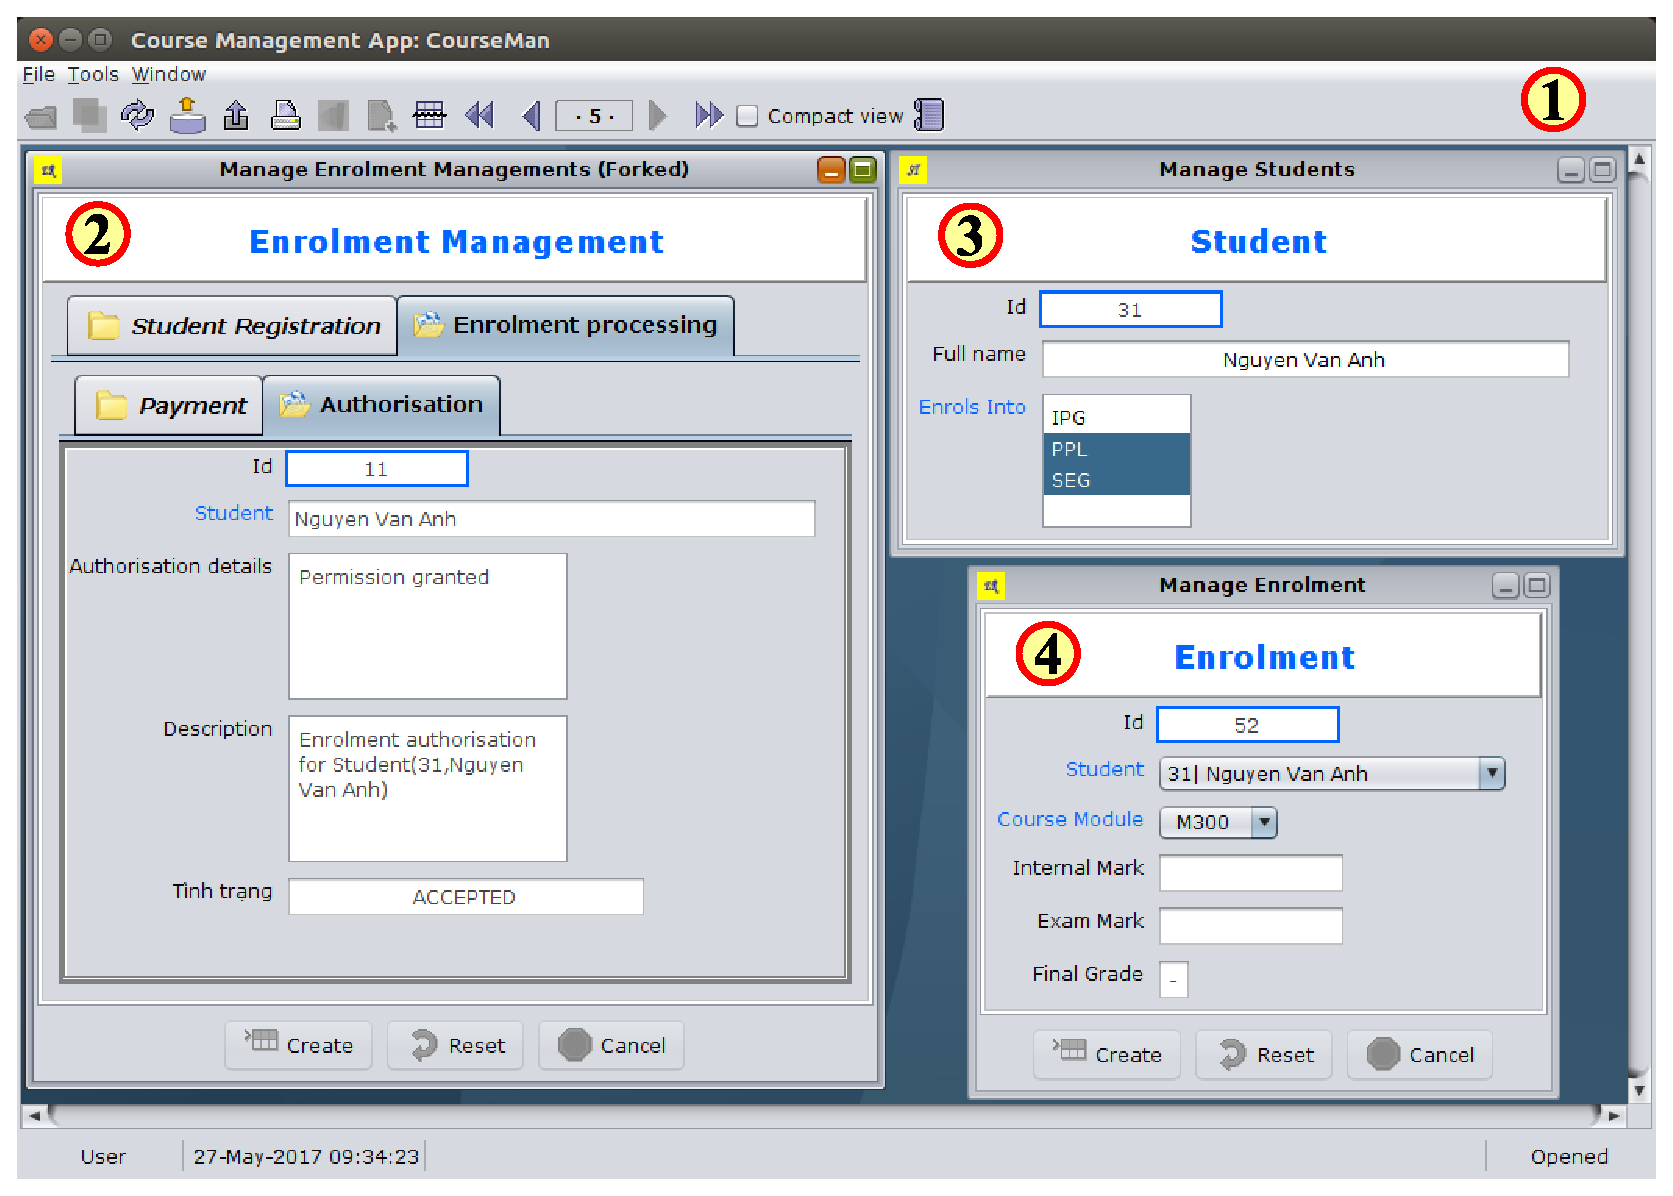
\includegraphics[scale=0.5]{software-tool}
%	\caption{The GUI of \courseman~software prototype generated in Java: (1) desktop, 
%		(2-4) the object UIs of \clazz{EnrolmentMgmt}, \clazz{Student}, and \clazz{Enrolment}.} %
%	\label{fig:software-tool}
%\end{figure*}
%
%Figure~\ref{fig:software-tool} shows the GUI of a \courseman~software that is generated automatically by our Java tool. We adapted this GUI from the description in~\cite{le_domain_2018}.
